% ============================================================
% M3 S2 导学件·波1 片件 —— 课时18 2.8②压轴综合二（母版照抄制·补位臂4b）
% 生成：M3 成卷轮 S2 波1 补位臂4b｜2026-09-14｜编译 cwd＝本目录（中文路径禁 \input 绝对路径）
%   xelatex main-true.tex ×2 → 含详解印本；xelatex main-false.tex ×2 → 纯题版（单源双本）
% 输入链（全只读）：题面库 课时18-2.8②压轴综合二.md（题面逐字装配）＋ -答案侧.md（值逐字回嵌）
%   ＋ 定稿/批E-课时18-2.8②压轴综合二.md（详解回嵌源＝§七 补产 16 块【详解】＋件末「导学 G5 补产」5 键；
%   G1 已承 0914 撤换回冲后版本＝3章件17-#19）；
%   toolchain＝qp-m3.sty（钉后版 md5 7c3930362be8a0a2bdf21bbf8ac16573，本地挂载副本，破损即停）。
% 母版体例：详见 成卷/导学件/课时01-坐标法/母版体例说明.md（骨架/宏用法/门谱/坑）。
% 键账：件内 ansblock 键集 ≡ 题面库片键集 ≡ manifest 键序（21 键，零缺漏零多余）；
%   预习位零键零答案；印面号 1—21＝探究 1—16＋课堂评价 17—21，键↔号映射见 值台账-课时18.json。
% 多选门：本片多选 1 道（18-02，印12）≤4 合规，成卷未增；印面带 \duoxuan\hspace{0.6em} 标记。
% 印面符号口径：源详解 ⇒ 箭头改「得/即」文读、✓/✗ 改「符合/不合」文读、〔亲算印证〕〔闸注〕
%   源注不入印面；18-06 详解 k₁k₂ 化简笔误（源 −k²−4k）经亲算复算订正为 −4k（结论不变，台账留痕）；
%   18-03 值行 S_max、19 片值行下标遇文本态下划线字符，经 \catcode 组内局部化照字印出（值字节零改动）。
% 括线判据（承重墙禁放宽）：估高＞8 行（chars/23 栏宽口径）→ 括线模，逐键读数入值台账；
%   其余灰底。本片括线键以门谱读数为准（20 键括线＋G4 灰底，见值台账判模口径）。
% 门谱读数：见 过程件 工作区/_tmpM3S2波1补位4b_0914/（编译 log、门谱输出、台账）。
% ============================================================
\documentclass[fontset=none]{ctexart}
\usepackage{qp-m3}
% —— 印面逐字符号路由补钉（探针实证 0914：书宋缺 U+2212，▱ 诸字库皆缺→NSC 子块；
%     禁改 sty 本体保 md5；无 ▱/− 用件的片可整块照抄，零副作用） ——
\xeCJKDeclareCharClass{Default}{"2212}%
\setCJKfamilyfont{nscblk}[Path=C:/提示词/工作区/字替对照-0909/variantF/fonts/,BoldFont=NSC-w600.ttf]{NSC-w500.ttf}%
\xeCJKDeclareSubCJKBlock{nscblk}{"25B1}%
\newcommand{\pxparallelogram}{{\CJKfamily{nscblk}▱}}%
% —— 断行微调（纯题档/详解档三零门：CJK 胶收缩 0.01→0.05em；应急伸展撤行回落 sty 默认
%     1em 三零仍守（母版 2026-09-14 实测），补丁最少化；Underfull 治理读数见过程件） ——
\xeCJKsetup{CJKglue={\hskip 0.10em plus 0.08em minus 0.05em}}%
% —— 页脚件名（qp-headfoot 复用入口） ——
\renewcommand{\qpzhangming}{第二章\quad 平面解析几何}%
\renewcommand{\qpjianming}{导学件}%

\begin{document}

\zhangtitle{第二章\quad 平面解析几何}
\jietitle{2.8 直线与圆锥曲线的位置关系（二）}
\mubiaoline
\mubiaomu{1}{掌握直线与椭圆、双曲线、抛物线位置关系的判定方法，会联立方程后用判别式与根与系数的关系处理交点与弦长问题，能识别并处理直线与渐近线、对称轴平行的退化情形；}
\mubiaomu{2}{掌握弦长公式与中点弦点差法，会用设线设点把定点、定值、存在性条件化为坐标运算，形成“设参—化简—回验”的规范求解路径；}
\mubiaomu{3}{会求向量数量积约束下的面积与最值问题，体会方程思想、函数思想与转化化归思想在压轴综合问题中的运用价值.}

\vspace{1.7mm}
\begin{multicols}{2}
\emergencystretch=1em

% ============================================================
% 课前预习（知识点导学填空；零键零答案——\kongbai 空线＋\zhentib 判断题面形，
% 两档等形不泄答）
% ============================================================
\huaxing{课}{前}{预}{习}{知识导学\quad 素养初识}

\zsd{一}{位置关系判定与弦问题}

\tiaomu{1}{直线与圆锥曲线位置关系的判定：联立方程消元得一元方程，相交、相切、相离分别对应\kongbai{}；二次项系数含参数时，须先讨论系数为零的退化情形（直线与渐近线或对称轴平行）．\zhuzhu{消元后 \(\Delta>0\) 两交点、\(\Delta=0\) 恰一交点、\(\Delta<0\) 无交点；双曲线、抛物线还要单列一次方程情形，交点个数与相切不等价.}}

\tiaomu{2}{弦长公式：直线\(y=kx+b\)（\(k\) 存在）与曲线交于\(A(x_1,y_1)\)、\(B(x_2,y_2)\)两点，则\(|AB|=\)\kongbai{}；中点弦问题可用点差法求斜率，但求出后须回验\kongbai{}．\zhuzhu{根与系数的关系是弦长与中点弦的共同工具；点差法解出的斜率必须代回判别式检验弦存在，防“无弦之弦”.}}

\zsd{二}{定点、定值与存在性}

\tiaomu{1}{定点（定值）问题：设出直线或点的参数，把目标量表示为参数式，化简后若参数\kongbai{}，则对一切允许参数结论成立；存在性问题先\kongbai{}，解出后代回检验．\zhuzhu{定点常在坐标轴上，可先由特殊位置猜出再一般证明；存在性设参求解后必须回代验证，越界根舍、退化情形单列讨论.}}

\zsd{三}{面积与最值}

\tiaomu{1}{弦与顶点构成的三角形面积常取\kongbai{}为底，化归为纵坐标差（或点到直线距离）的运算；最值问题把目标表示为单一参数的函数后求最值，并检验取等条件落在允许范围内．\zhuzhu{抛物线焦点弦有现成公式可用；面积最值注意判别式对参数范围的截断，取等点不在定义域内时应在端点比较.}}

\zhenhead{判断正误(正确的打\gou{},错误的打\cha{})}

\zhentib{(1)}{直线与抛物线只有一个公共点时，直线与该抛物线一定相切．}

\zhentib{(2)}{用点差法求出中点弦所在直线的斜率后，不需要再检验直线与曲线是否相交．}

\liubai[9mm]{此处书写}

% ============================================================
% 课中探究（考点探究〔例+变式〕＝练槽 16 键；题后紧跟答案＝ansblock 内嵌，
% 值照答案侧逐字，详解承批E §七【详解】/「导学 G5 补产」回嵌＋印面清洗）
% ============================================================
\huaxing{课}{中}{探}{究}{考点探究\quad 素养小结}

% ---------- 探究点一 存在性、定点与定比构造（印面 1—6） ----------
\tjdnr{一}{存在性、定点与定比构造}{例\textbf{1}}{中档(知识点二)}{设双曲线\(E\)：\(x^{2}-y^{2}/3=1\)的左、右焦点为\(F_1\)、\(F_2\)，左顶点为\(A\)，点\(M\)是双曲线\(E\)在第一象限内的一点，直线\(MF_1\)交双曲线\(E\)的左支于点\(N\)，若\(NA\parallel MF_2\)，则\(|MF_2|=\)\nobreak(\kongwei)}

\bindopt {\fontsize{10.5pt}{\qpTJgLeadLiti}\selectfont \makebox[\dimexpr0.25\linewidth-0.5em\relax][l]{A．\(7/4\)}\makebox[\dimexpr0.25\linewidth-0.5em\relax][l]{B．\(5/2\)}\makebox[\dimexpr0.25\linewidth-0.5em\relax][l]{C．\(8/3\)}\makebox[\dimexpr0.25\linewidth-0.5em\relax][l]{D．\(11/4\)}\par}

{\ansblockgrayfalse
\begin{ansblock}[2章-练-课时18-01]
% ans:2章-练-课时18-01
\ansitem{1}{B（|MF₂|=5/2）}
\ansnote{详解}{\(F_1(-2,0)\)、\(F_2(2,0)\)、\(A(-1,0)\)，故 \(F_1A/F_1F_2=1/4\)．\(NA\parallel MF_2\)，得 \(\triangle F_1AN\sim\triangle F_1MF_2\)，故 \(F_1N/F_1M=1/4\)．设 \(M(x_0,y_0)\)（\(x_0>0\)，\(y_0>0\)），则 \(N=F_1+(1/4)(M-F_1)=((x_0-6)/4,y_0/4)\)．\(M\)、\(N\) 均在 \(E\) 上：\(x_0^{2}-y_0^{2}/3=1\)，且 \(((x_0-6)/4)^{2}-(y_0/4)^{2}/3=1\)，后者乘16得 \((x_0-6)^{2}-y_0^{2}/3=16\)；两式相减 \((x_0-6)^{2}-x_0^{2}=15\)，即 \(-12x_0+36=15\)，解得 \(x_0=7/4\)，进而 \(y_0^{2}=3(x_0^{2}-1)=99/16\)，\(y_0=3\sqrt{11}/4\)．于是 \(|MF_2|=\sqrt{(7/4-2)^{2}+99/16}=\sqrt{100/16}=5/2\)．故选：B．}
\end{ansblock}}

\liB{变式\textbf{2}}{中档(知识点二)}{}{焦距为\(2c\)的椭圆\(\Gamma\)：\(x^{2}/a^{2}+y^{2}/b^{2}=1\)（\(a>b>0\)），如果满足「\(2b=a+c\)」，则称此椭圆为「等差椭圆」．}

\bindp (1) 如果椭圆\(\Gamma\)是「等差椭圆」，求\(b/a\)的值；

\bindp (2) 对于焦距为12的「等差椭圆」，点\(A\)为椭圆短轴的上顶点，\(P\)为椭圆上异于\(A\)点的任一点，\(Q\)为\(P\)关于原点\(O\)的对称点（\(Q\)也异于\(A\)），直线\(AP\)、\(AQ\)分别与\(x\)轴交于\(M\)、\(N\)两点，判断以线段\(MN\)为直径的圆是否过定点？说明理由．
\xiexwei{18mm}

{\ansblockgrayfalse
\begin{ansblock}[2章-练-课时18-07]
% ans:2章-练-课时18-07
\ansitem{2}{(1) 4/5；(2) 恒过定点 (0,±10)}
\ansnote{详解}{(1) 由 \(2b=a+c\) 得 \(c=2b-a\)，代入 \(c^{2}=a^{2}-b^{2}\)：\((2b-a)^{2}=a^{2}-b^{2}\)，展开得 \(4b^{2}-4ab=0\)，故 \(b/a=4/5\)．\par\noindent (2) \(2c=12\)，故 \(c=6\)；由 \(b^{2}=16a^{2}/25\) 与 \(a^{2}-b^{2}=36\) 得 \(9a^{2}/25=36\)，故 \(a^{2}=100\)、\(b^{2}=64\)，\(A(0,8)\)．设 \(P(x_0,y_0)\)（\(x_0\neq 0\)），则 \(Q(-x_0,-y_0)\)．直线 \(AP\)：\(y=(y_0-8)x/x_0+8\)，令 \(y=0\) 得 \(M(8x_0/(8-y_0),0)\)；同理 \(N(-8x_0/(8+y_0),0)\)．以 \(MN\) 为直径的圆：\((x-8x_0/(8-y_0))(x+8x_0/(8+y_0))+y^{2}=0\)，其 \(x\) 的交叉项 \(=8x_0[(8-y_0)-(8+y_0)]/(64-y_0^{2})=-16x_0y_0/(64-y_0^{2})\)．由 \(x_0^{2}/100+y_0^{2}/64=1\) 得 \(64-y_0^{2}=64x_0^{2}/100=16x_0^{2}/25\)，故圆方程化为 \(x^{2}+y^{2}-(25y_0/x_0)x-100=0\)．令 \(x=0\) 得 \(y=\pm 10\)，与 \(P\) 无关，故恒过定点 \((0,10)\) 与 \((0,-10)\)（\(P\) 异于 \(A\) 保证 \(x_0\neq 0\)、\(64-y_0^{2}>0\)）．}
\end{ansblock}}

\tjdnr{一}{存在性、定点与定比构造}{例\textbf{3}}{中档(知识点二)}{已知圆\(A\)：\(x^{2}+y^{2}+2x-15=0\)和定点\(B(1,0)\)，\(M\)是圆\(A\)上任意一点，线段\(MB\)的垂直平分线交\(MA\)于点\(N\)，设点\(N\)的轨迹为\(C\)．}

\bindp (1) 求\(C\)的方程；

\bindp (2) 若直线\(y=k(x-1)\)与曲线\(C\)相交于\(P\)、\(Q\)两点，试问：在\(x\)轴上是否存在定点\(R\)，使当\(k\)变化时，总有\(\angle ORP=\angle ORQ\)？若存在，求出点\(R\)的坐标；若不存在，请说明理由．
\xiexwei{18mm}

{\ansblockgrayfalse
\begin{ansblock}[2章-练-课时18-08]
% ans:2章-练-课时18-08
\ansitem{3}{(1) x²/4+y²/3=1；(2) 存在，R(4,0)}
\ansnote{详解}{(1) 圆 \(A\) 即 \((x+1)^{2}+y^{2}=16\)，圆心 \(A(-1,0)\)、半径4．由垂直平分线性质得 \(|NM|=|NB|\)，而 \(N\) 在 \(MA\) 上，故 \(|NA|+|NB|=|NA|+|NM|=|MA|=4>|AB|=2\)，轨迹为以 \(A\)、\(B\) 为焦点的椭圆：\(2a=4\)、\(2c=2\)，即 \(a^{2}=4\)、\(b^{2}=3\)，故 \(C\)：\(x^{2}/4+y^{2}/3=1\)．\par\noindent (2) 设 \(R(t,0)\)．联立得 \((4k^{2}+3)x^{2}-8k^{2}x+4k^{2}-12=0\)，故 \(x_1+x_2=8k^{2}/(4k^{2}+3)\)、\(x_1x_2=(4k^{2}-12)/(4k^{2}+3)\)．\(\angle ORP=\angle ORQ\) 等价于 \(k_{RP}+k_{RQ}=0\)，即 \(y_1/(x_1-t)+y_2/(x_2-t)=0\)．以 \(y_i=k(x_i-1)\) 代入，分子 \(=k[2x_1x_2-(1+t)(x_1+x_2)+2t]=0\)；\(k\neq 0\) 时即 \(2(4k^{2}-12)-8k^{2}(1+t)+2t(4k^{2}+3)=0\)，展开得 \(6t-24=0\)，故 \(t=4\)（\(k=0\) 时 \(P\)、\(Q\) 为长轴两端点，等式显然成立）．故存在 \(R(4,0)\)，与 \(k\) 无关．}
\end{ansblock}}

\liB{变式\textbf{4}}{中档(知识点二)}{}{过双曲线\(x^{2}/a^{2}-y^{2}/3=1\)（\(a>0\)）的右焦点\(F\)作直线\(l\)与双曲线交于\(A\)、\(B\)两点，使得\(|AB|=6\)，若这样的直线有且只有两条，则实数\(a\)的取值范围是\nobreak(\kongwei)}

\bindopt {\fontsize{10.5pt}{\qpTJgLeadLiti}\selectfont \makebox[\dimexpr0.5\linewidth-1em\relax][l]{A．\((0,1]\cup(3,+\infty)\)}\makebox[\dimexpr0.5\linewidth-1em\relax][l]{B．\((0,1)\cup(3,+\infty)\)}\par}

\bindopt {\fontsize{10.5pt}{\qpTJgLeadLiti}\selectfont \makebox[\dimexpr0.5\linewidth-1em\relax][l]{C．\((0,1)\)}\makebox[\dimexpr0.5\linewidth-1em\relax][l]{D．\((3,+\infty)\)}\par}

{\ansblockgrayfalse
\begin{ansblock}[2章-练-课时18-10]
% ans:2章-练-课时18-10
\ansitem{4}{B}
\ansnote{详解}{过焦点的弦分两型：跨支型（\(A\)、\(B\) 各在一支）弦长下限为 \(2a\)，且实轴所在直线（长 \(2a\)）恰1条，长 \(L>2a\) 时对称地有2条；单支型（同在右支）弦长下限为通径 \(2b^{2}/a=6/a\)，通径（\(l\perp x\) 轴）恰1条，\(L>6/a\) 时有2条．且 \(6/a\) 与 \(2a\) 不可能同时等于6（\(a=1\) 时 \(6/a=6\)、\(2a=2\)；\(a=3\) 时 \(2a=6\)、\(6/a=2\)）．令 \(L=6\) 分段计数：\(a<1\) 时跨支 \(6>2a\) 有2条、单支 \(6<6/a\) 有0条，合计2，符合；\(a=1\) 时 \(2+1=3\)，不合；\(1<a<3\) 时 \(2+2=4\)，不合；\(a=3\) 时 \(1+2=3\)，不合；\(a>3\) 时跨支 \(6<2a\) 有0条、单支 \(6>6/a\) 有2条，合计2，符合．故 \(a\in(0,1)\cup(3,+\infty)\)，选 B．}
\end{ansblock}}

\tjdnr{一}{存在性、定点与定比构造}{例\textbf{5}}{难(知识点二)}{已知椭圆\(C\)：\(x^{2}/a^{2}+y^{2}/b^{2}=1\)（\(a>b>0\)）的离心率为\(\sqrt{2}/2\)，椭圆的右焦点与右顶点及上顶点构成的三角形面积为\(\sqrt{2}-1\)．}

\bindp (1) 求椭圆\(C\)的标准方程；

\bindp (2) 已知直线\(y=k(x-1)\)与椭圆\(C\)交于\(A\)、\(B\)两点，若点\(Q\)的坐标为\((7/4,0)\)，问：是否存在\(k\)，使得\(QA\cdot QB>1\)？若存在，求出\(k\)的取值范围；不存在，请说明理由．
\xiexwei{18mm}

{\ansblockgrayfalse
\begin{ansblock}[2章-练-课时18-11]
% ans:2章-练-课时18-11
\ansitem{5}{(1) x²/4+y²/2=1；(2) 不存在（QA·QB≡−15/16 恒<1）}
\ansnote{详解}{(1) \(e=\sqrt{2}/2\)，故 \(a^{2}=2c^{2}\)、\(b^{2}=c^{2}\)；三角形面积 \(=(a-c)b/2=(\sqrt{2}-1)c^{2}/2=\sqrt{2}-1\)，得 \(c^{2}=2\)，故 \(a^{2}=4\)、\(b^{2}=2\)，椭圆 \(C\)：\(x^{2}/4+y^{2}/2=1\)．\par\noindent (2) 直线过 \((1,0)\)（椭圆内一点），恒有两交点．联立得 \((1+2k^{2})x^{2}-4k^{2}x+2k^{2}-4=0\)，故 \(x_1+x_2=4k^{2}/(1+2k^{2})\)、\(x_1x_2=(2k^{2}-4)/(1+2k^{2})\)；\(y_1y_2=k^{2}(x_1-1)(x_2-1)=-3k^{2}/(1+2k^{2})\)．于是 \(QA\cdot QB=(x_1-7/4)(x_2-7/4)+y_1y_2=x_1x_2-(7/4)(x_1+x_2)+49/16+y_1y_2\)，代入化简 \(=[(2k^{2}-4)-7k^{2}-3k^{2}]/(1+2k^{2})+49/16=(-8k^{2}-4)/(1+2k^{2})+49/16=-4+49/16=-15/16\)，与 \(k\) 无关且恒小于1，故不存在这样的 \(k\)．}
\end{ansblock}}

\liB{变式\textbf{6}}{难(知识点二)}{}{在平面直角坐标系\(xOy\)中，已知椭圆\(C\)：\(x^{2}/a^{2}+y^{2}/b^{2}=1\)（\(a>b>0\)），\(F\)是椭圆的右焦点且\kongbai{}，从下列条件中任选一个补充在上面问题中并作答（注：如果选择多个条件作答，按第一个计分）．}

\bindp 条件①：椭圆\(C\)的离心率\(e=1/2\)，焦点到相应准线的距离是3；

\bindp 条件②：椭圆\(C\)与圆\(M\)：\((x-6)^{2}+y^{2}=16\)外切，又与圆\(N\)：\(x^{2}+(y-2\sqrt{3})^{2}=3\)外切．

\bindp (1) 求椭圆\(C\)的方程；

\bindp (2) 已知\(A\)、\(B\)是椭圆\(C\)上关于原点对称的两点，\(A\)在\(x\)轴的上方，连接\(AF\)、\(BF\)并分别延长交椭圆\(C\)于\(D\)、\(E\)两点，证明：直线\(DE\)过定点．
\xiexwei{18mm}

{\ansblockgrayfalse
\begin{ansblock}[2章-练-课时18-09]
% ans:2章-练-课时18-09
\ansitem{6}{(1) 两条件均得 x²/4+y²/3=1；(2) DE 恒过定点 (8/5,0)}
\ansnote{详解}{(1) 条件①：\(e=1/2\)，故 \(a=2c\)；焦点到相应准线距离 \(a^{2}/c-c=3\)，即 \(4c-c=3\)，得 \(c=1\)，故 \(a^{2}=4\)、\(b^{2}=3\)．条件②：\(\odot M\) 圆心 \((6,0)\)、半径4，椭圆在圆内一侧外切，切点必为右顶点，故 \(a+4=6\)，\(a=2\)；\(\odot N\) 圆心 \((0,2\sqrt{3})\)、半径 \(\sqrt{3}\)，故 \(b=\sqrt{3}\)、\(b^{2}=3\)．回验唯一性（外切即恰一公共点）：\(\odot M\) 与椭圆联立消 \(y\) 得 \(x^{2}-48x+92=0\)，\(x=2\) 或 \(x=46\)（46越界，舍）；\(\odot N\) 联立得 \(y^{2}+12\sqrt{3}y-39=0\)，\(y=\sqrt{3}\) 或 \(y=-13\sqrt{3}\)（越界，舍）．两条件同得 \(x^{2}/4+y^{2}/3=1\)．\par\noindent (2) \(F(1,0)\)．设 \(A(x_1,y_1)\)（\(y_1>0\)）、\(B(-x_1,-y_1)\)，满足 \(3x_1^{2}+4y_1^{2}=12\)．直线 \(AF\)：\(x=my+1\)（\(m=(x_1-1)/y_1\)），直线 \(BF\)：\(x=ny+1\)（\(n=(x_1+1)/y_1\)），则 \(n-m=2/y_1\)．\(x=my+1\) 代入 \(3x^{2}+4y^{2}=12\)：\((3m^{2}+4)y^{2}+6my-9=0\)，故 \(y_1y_D=-9/(3m^{2}+4)\)，即 \(y_D=-9/[(3m^{2}+4)y_1]\)；同理 \(y_E=9/[(3n^{2}+4)y_1]\)，且 \(x_D=my_D+1\)、\(x_E=ny_E+1\)．\par\noindent \(D\)、\(E\)、\(P(8/5,0)\) 三点共线等价于 \(y_D(x_E-8/5)=y_E(x_D-8/5)\)，即 \(y_Dy_E(n-m)=(3/5)(y_D-y_E)\)（记为①）．代入 \(y_Dy_E=-81/[(3m^{2}+4)(3n^{2}+4)y_1^{2}]\) 与 \(y_D-y_E=-(9/y_1)(3m^{2}+3n^{2}+8)/[(3m^{2}+4)(3n^{2}+4)]\)，则①等价于 \(30/y_1^{2}=3(m^{2}+n^{2})+8\)，即 \(30=3y_1^{2}(m^{2}+n^{2})+8y_1^{2}=3[(x_1-1)^{2}+(x_1+1)^{2}]+8y_1^{2}=6x_1^{2}+6+8y_1^{2}=2(3x_1^{2}+4y_1^{2})+6=24+6=30\)，恒成立．故 \(DE\) 恒过定点 \((8/5,0)\)．}
\end{ansblock}}

\xiaojie{①识别：以弦长条数反求参数（跨支/单支分段计数）、向量积恒值否定存在性、以弦为直径的圆过定点、定比构造求焦半径等为目标的题，判归本题型．}
\bindp {\kaishu ②操作：先定型（跨支/单支、何为下界弦），按对称性计数；定点定值设线设参，把几何条件译成坐标等式后化简，让参数自然消去；存在性设参求解后必须回代检验．}
\bindp {\kaishu ③收束：分段计数逐段核对恰“有且只有”的条数；定点结论须带回验（特例或恒等式），退化与越界根要单独交代．}

% ---------- 探究点二 面积、定值与最值（印面 7—11） ----------
\tjdnr{二}{面积、定值与最值}{例\textbf{7}}{难(知识点三)}{设抛物线\(y^{2}=2px\)（\(p>0\)）的焦点为\(F\)，点\(F\)到抛物线准线的距离为2．若椭圆\(x^{2}/a^{2}+y^{2}/b^{2}=1\)（\(a>b>0\)）的右焦点也为\(F\)，离心率为\(1/2\)．}

\bindp (1) 求抛物线方程和椭圆方程；

\bindp (2) 若不经过\(F\)的直线\(l\)与抛物线交于\(A\)、\(B\)两点，且\(OA\cdot OB=-3\)（\(O\)为坐标原点），直线\(l\)与椭圆交于\(C\)、\(D\)两点，求\(\triangle CDF\)面积的最大值．
\xiexwei{18mm}

{\ansblockgrayfalse
\begin{ansblock}[2章-练-课时18-03]
% ans:2章-练-课时18-03
{\catcode`\_=12 \ansitem{7}{(1) y²=4x、x²/4+y²/3=1；(2) S_max=2√3/3}}
\ansnote{详解}{(1) 焦点到准线的距离 \(p=2\)，故抛物线 \(y^{2}=4x\)，\(F(1,0)\)；椭圆 \(c=1\)、\(e=c/a=1/2\)，故 \(a=2\)、\(b^{2}=a^{2}-c^{2}=3\)，椭圆 \(x^{2}/4+y^{2}/3=1\)．\par\noindent (2) 设 \(l\)：\(x=my+n\)（不过 \(F\)，故 \(n\neq 1\)）．交抛物线：\(y^{2}-4my-4n=0\)，得 \(y_1y_2=-4n\)、\(x_1x_2=(y_1y_2)^{2}/16=n^{2}\)．由 \(OA\cdot OB=n^{2}-4n=-3\) 得 \(n=1\)（此时 \(l\) 过 \(F(1,0)\)，舍）或 \(n=3\)．交椭圆：\(3(my+3)^{2}+4y^{2}=12\)，即 \((3m^{2}+4)y^{2}+18my+15=0\)，\(\Delta=144m^{2}-240\geqslant 0\)，故 \(m^{2}\geqslant 5/3\)．\(l\) 交 \(x\) 轴于 \(T(3,0)\)，\(|TF|=2\)，故 \(S_{\triangle CDF}=|TF|\cdot|y_C-y_D|/2=|y_C-y_D|\)，\(S^{2}=(144m^{2}-240)/(3m^{2}+4)^{2}\)．令 \(u=3m^{2}+4\)（\(u\geqslant 9\)）：\(S^{2}=48/u-432/u^{2}\)；再令 \(v=1/u\in(0,1/9]\)：\(S^{2}=48v-432v^{2}\) 在 \(v=1/18\) 处取最大（\(1/18\in(0,1/9]\)），\(S^{2}\) 最大值为 \(48/18-432/324=4/3\)，故 \(S\) 的最大值为 \(2\sqrt{3}/3\)，此时 \(3m^{2}+4=18\)，\(m^{2}=14/3\)，满足 \(m^{2}\geqslant 5/3\)．}
\end{ansblock}}

\liB{变式\textbf{8}}{难(知识点三)}{}{已知椭圆\(x^{2}+2y^{2}=1\)，过原点的两条直线\(l_1\)和\(l_2\)分别与椭圆交于\(A\)、\(B\)和\(C\)、\(D\)，记得到的平行四边形\(ACBD\)的面积为\(S\)．}

\bindp (1) 设\(A(x_1,y_1)\)、\(C(x_2,y_2)\)，用\(A\)、\(C\)的坐标表示点\(C\)到直线\(l_1\)的距离，并证明\(S=2|x_1y_2-x_2y_1|\)；

\bindp (2) 从①②两个问题中任选一个作答：①设\(l_1\)与\(l_2\)的斜率之积为\(-1/2\)，求面积\(S\)的值；②设\(l_1\)与\(l_2\)的斜率之积为\(m\)，求\(m\)的值，使得无论\(l_1\)与\(l_2\)如何变动，面积\(S\)保持不变．
\xiexwei{18mm}

{\ansblockgrayfalse
\begin{ansblock}[2章-练-课时18-04]
% ans:2章-练-课时18-04
\ansitem{8}{(1) d=|x₁y₂−x₂y₁|/√(x₁²+y₁²)，证毕；①S=√2；②m=−1/2（此时 S≡√2）}
\ansnote{详解}{(1) \(l_1\)：\(y_1x-x_1y=0\)（\(x_1=0\) 时即 \(x=0\)，公式仍适用），故 \(d=|y_1x_2-x_1y_2|/\sqrt{x_1^{2}+y_1^{2}}\)．\(O\) 同时平分 \(AB\) 与 \(CD\)，故 \(S=4S_{\triangle OAC}=4\cdot|OA|\cdot d/2=2\sqrt{x_1^{2}+y_1^{2}}\cdot|x_1y_2-x_2y_1|/\sqrt{x_1^{2}+y_1^{2}}=2|x_1y_2-x_2y_1|\)，得证．\par\noindent (2) 记 \(y_i=k_ix_i\)，则 \(x_i^{2}=1/(1+2k_i^{2})\)，\(S=2|x_1||x_2||k_2-k_1|=2|k_2-k_1|/\sqrt{(1+2k_1^{2})(1+2k_2^{2})}\)．\par\noindent ① \(k_1k_2=-1/2\)：分母 \(=(1+2k_1^{2})(1+2k_2^{2})=1+2(k_1^{2}+k_2^{2})+4k_1^{2}k_2^{2}=2(1+k_1^{2}+k_2^{2})\)；\((k_2-k_1)^{2}=k_1^{2}+k_2^{2}-2k_1k_2=1+k_1^{2}+k_2^{2}\)，故 \(S^{2}=4(1+k_1^{2}+k_2^{2})/[2(1+k_1^{2}+k_2^{2})]=2\)，即 \(S=\sqrt{2}\)．\par\noindent ② 记 \(T=k_1^{2}+k_2^{2}\)，则 \((k_2-k_1)^{2}=T-2m\)、分母 \(=2T+1+4m^{2}\)，\(S^{2}=4(T-2m)/(2T+1+4m^{2})\)．要与 \(T\) 无关，须存在 \(\lambda\) 使 \(T-2m\equiv\lambda(2T+1+4m^{2})\)：比较系数得 \(2\lambda=1\)、\(\lambda(1+4m^{2})=-2m\)，故 \((1+4m^{2})/2=-2m\)，即 \(4m^{2}+4m+1=0\)，解得 \(m=-1/2\)（与①自洽，此时对一切 \(T\) 有 \(S^{2}=2\)）．}
\end{ansblock}}

\tjdnr{二}{面积、定值与最值}{例\textbf{9}}{中档(知识点三)}{已知抛物线\(G\)：\(y^{2}=4x\)的焦点与椭圆\(E\)：\(x^{2}/a^{2}+y^{2}/b^{2}=1\)（\(a>b>0\)）的右焦点\(F\)重合，椭圆\(E\)的长轴长为4．}

\bindp (1) 求椭圆\(E\)的方程；

\bindp (2) 过点\(F\)且斜率为\(k\)的直线\(l\)交椭圆\(E\)于\(A\)、\(B\)两点，交抛物线\(G\)于\(M\)、\(N\)两点，请问是否存在实常数\(t\)，使\(2/|AB|+t/|MN|\)为定值？若存在，求出\(t\)的值；若不存在，说明理由．
\xiexwei{18mm}

{\ansblockgrayfalse
\begin{ansblock}[2章-练-课时18-05]
% ans:2章-练-课时18-05
\ansitem{9}{(1) x²/4+y²/3=1；(2) 存在，t=−2/3，定值 1/2}
\ansnote{详解}{(1) \(y^{2}=4x\) 的焦点为 \((1,0)\)，故 \(c=1\)；长轴 \(2a=4\)，故 \(a=2\)、\(b^{2}=3\)，椭圆 \(E\)：\(x^{2}/4+y^{2}/3=1\)．\par\noindent (2) \(l\)：\(y=k(x-1)\)（\(k\neq 0\)）．交椭圆：\((3+4k^{2})x^{2}-8k^{2}x+4k^{2}-12=0\)，故 \(|AB|=\sqrt{1+k^{2}}\cdot\sqrt{(x_1+x_2)^{2}-4x_1x_2}=12(1+k^{2})/(3+4k^{2})\)．交抛物线：\(k^{2}x^{2}-(2k^{2}+4)x+k^{2}=0\)，故 \(x_3+x_4=(2k^{2}+4)/k^{2}\)，\(|MN|=x_3+x_4+2=4(1+k^{2})/k^{2}\)（焦点弦）．于是 \(2/|AB|+t/|MN|=(3+4k^{2})/(6(1+k^{2}))+tk^{2}/(4(1+k^{2}))=[(8+3t)k^{2}+6]/(12(1+k^{2}))\)，与 \(k\) 无关等价于 \(8+3t=6\)，故 \(t=-2/3\)，此时定值为 \(6/12=1/2\)．}
\end{ansblock}}

\liB{变式\textbf{10}}{中档(知识点三)}{}{已知抛物线\(C\)：\(y^{2}=-4x\)，直线\(l\)过定点\(P(0,1)\)．}

\bindp (1) 若\(l\)与\(C\)仅有一个公共点，求直线\(l\)的方程；

\bindp (2) 若\(l\)与\(C\)交于\(A\)、\(B\)两点，直线\(OA\)、\(OB\)（\(O\)为坐标原点）的斜率分别为\(k_1\)、\(k_2\)，试探究在\(k_1-k_2\)、\(k_1+k_2\)、\(k_1/k_2\)、\(k_1k_2\)中，运算结果是否为定值？并说明理由．
\xiexwei{14mm}

{\ansblockgrayfalse
\begin{ansblock}[2章-练-课时18-06]
% ans:2章-练-课时18-06
\ansitem{10}{(1) y=1 或 x=0 或 y=−x+1；(2) 仅 k₁+k₂=−4 为定值，其余三个均不是}
\ansnote{详解}{(1) 分三类：与对称轴（\(x\) 轴）平行的直线 \(y=1\)，恰一公共点；过顶点的切线 \(x=0\)；斜线 \(y=kx+1\)（\(k\neq 0\)）代入得 \(k^{2}x^{2}+(2k+4)x+1=0\)，令 \(\Delta=(2k+4)^{2}-4k^{2}=16k+16=0\)，得 \(k=-1\)，即 \(y=-x+1\)．共三条．\par\noindent (2) 有两交点，故 \(k\) 存在、\(k\neq 0\) 且 \(\Delta=16k+16>0\)，即 \(k>-1\)．联立 \(k^{2}x^{2}+(2k+4)x+1=0\)，得 \(x_1+x_2=-(2k+4)/k^{2}\)、\(x_1x_2=1/k^{2}\)．\(k_i=y_i/x_i=k+1/x_i\)：\(k_1+k_2=2k+(x_1+x_2)/(x_1x_2)=2k-(2k+4)=-4\)，为定值；\(k_1k_2=y_1y_2/(x_1x_2)=-4k\)，随 \(k\) 变；\(|k_1-k_2|=|x_2-x_1|/|x_1x_2|=4\sqrt{k+1}\)，随 \(k\) 变；\(k_1/k_2\) 同理随 \(k\) 变．故仅 \(k_1+k_2=-4\) 为定值．}
\end{ansblock}}

\tjdnr{二}{面积、定值与最值}{例\textbf{11}}{难(知识点三)}{已知椭圆\(E\)：\(x^{2}/a^{2}+y^{2}/b^{2}=1\)（\(a>b>0\)）的左、右焦点分别为\(F_1\)、\(F_2\)，离心率为\(e=\sqrt{3}/2\)，过左焦点\(F_1\)作直线\(l_1\)交椭圆\(E\)于\(A\)、\(B\)两点，\(\triangle ABF_2\)的周长为8．}

\bindp (1) 求椭圆\(E\)的方程；

\bindp (2) 若直线\(l_2\)：\(y=kx+m\)（\(km<0\)）与圆\(O\)：\(x^{2}+y^{2}=1\)相切，且与椭圆\(E\)交于\(M\)、\(N\)两点，\(|MF_2|+|NF_2|\)是否存在最小值？若存在，求出最小值和此时直线\(l_2\)的方程．
\xiexwei{18mm}

{\ansblockgrayfalse
\begin{ansblock}[2章-练-课时18-15]
% ans:2章-练-课时18-15
\ansitem{11}{(1) x²/4+y²=1；(2) 存在，min=2，此时 x−√2y−√3=0 或 x+√2y−√3=0}
\ansnote{详解}{(1) 周长 \(=|AB|+|AF_2|+|BF_2|=4a=8\)，故 \(a=2\)；\(e=\sqrt{3}/2\)，故 \(c=\sqrt{3}\)、\(b^{2}=1\)，椭圆 \(E\)：\(x^{2}/4+y^{2}=1\)．\par\noindent (2) 由相切得 \(d(O,l_2)=|m|/\sqrt{1+k^{2}}=1\)，即 \(m^{2}=1+k^{2}\)．焦半径公式（\(|x_i|\leqslant 2\) 保证非负）：\(|MF_2|=a-ex_M=2-(\sqrt{3}/2)x_M\)，同理 \(|NF_2|=2-(\sqrt{3}/2)x_N\)，故和 \(=4-(\sqrt{3}/2)(x_M+x_N)\)．联立 \(y=kx+m\) 与 \(x^{2}+4y^{2}=4\)：\((1+4k^{2})x^{2}+8kmx+4m^{2}-4=0\)，故 \(x_M+x_N=-8km/(1+4k^{2})\)；\(km<0\)，故 \(x_M+x_N=8\sqrt{k^{2}(1+k^{2})}/(1+4k^{2})\)．设 \(u=k^{2}>0\)，则 \(x_M+x_N=8\sqrt{u(1+u)}/(1+4u)\)；对 \(u(1+u)/(1+4u)^{2}\) 求导，分子正比于 \((1+2u)(1+4u)-8(u+u^{2})=1-2u\)，故 \(u=1/2\) 时最大，\(x_M+x_N\) 的最大值为 \(8\cdot(\sqrt{3}/2)/3=4\sqrt{3}/3\)，和的最小值为 \(4-(\sqrt{3}/2)\cdot(4\sqrt{3}/3)=2\)．此时 \(k^{2}=1/2\)、\(m^{2}=3/2\) 且 \(km<0\)，故 \((k,m)=(\sqrt{2}/2,-\sqrt{6}/2)\) 或 \((-\sqrt{2}/2,\sqrt{6}/2)\)，即 \(l_2\)：\(x-\sqrt{2}y-\sqrt{3}=0\) 或 \(x+\sqrt{2}y-\sqrt{3}=0\)．}
\end{ansblock}}

\xiaojie{①识别：以向量数量积（或斜率之积）为约束求面积最值、混合弦长定值反求参、多式辨定值、相切条件下焦半径和最值为目标的题，判归本题型．}
\bindp {\kaishu ②操作：面积取“弦交轴”截距段为底化归纵坐标差；定值辨析逐式表参数式看是否消参；最值先定参数范围（判别式、相切），再对一元函数求最值并回验取等．}
\bindp {\kaishu ③收束：向量垂直即数量积为零；焦点弦用定义或焦半径公式提速；结论必须带回原式核验（含退化情形与“恰一公共点”的排他检查）．}

% ---------- 探究点三 对称、多选与拼接综合（印面 12—16） ----------
\tjdnr{三}{对称、多选与拼接综合}{例\textbf{12}}{中档(知识点一)}{已知抛物线\(C\)：\(y^{2}=8x\)，\(O\)为坐标原点，其焦点为\(F\)，准线与\(x\)轴相交于\(M\)点，经过\(M\)点且斜率为\(k\)的直线\(l\)与抛物线相交于\(A(x_1,y_1)\)、\(B(x_2,y_2)\)两点，则下列结论中正确的是\nobreak(\kongwei)}

\lxopt{A．\(-1<k<1\)}

\lxopt{B．\(y_1y_2=8x_1x_2\)}

\lxopt{C．\(\angle AFB\)可能为直角}

\lxopt{D．当\(k^{2}=1/2\)时，\(\triangle AFB\)的面积为16}

{\ansblockgrayfalse
\begin{ansblock}[2章-练-课时18-02]
% ans:2章-练-课时18-02
\ansitem{12}{CD}
\ansnote{详解}{\(F(2,0)\)，准线 \(x=-2\)，故 \(M(-2,0)\)，\(l\)：\(y=k(x+2)\)．联立得 \(k^{2}x^{2}+(4k^{2}-8)x+4k^{2}=0\)；由两交点得 \(k^{2}\neq 0\) 且 \(\Delta=64(1-k^{2})>0\)，即 \(-1<k<1\) 且 \(k\neq 0\)，A 漏 \(k\neq 0\)，错．\par\noindent 改以 \(y\) 为主元：\(x=y^{2}/8\) 代入 \(l\) 得 \(ky^{2}-8y+16k=0\)，故 \(y_1+y_2=8/k\)、\(y_1y_2=16\)；而 \(x_1x_2=4\)，故 \(8x_1x_2=32\neq 16\)，B 错．\par\noindent \(FA\cdot FB=(x_1-2)(x_2-2)+y_1y_2=x_1x_2-2(x_1+x_2)+4+y_1y_2\)，其中 \(x_1+x_2=(8-4k^{2})/k^{2}\)，代入得 \(FA\cdot FB=32-16/k^{2}\)，当 \(k^{2}=1/2\) 时为0，故 \(\angle AFB\) 可为直角，C 对．\par\noindent \(S=|MF|\cdot|y_1-y_2|/2=2\sqrt{(y_1+y_2)^{2}-4y_1y_2}=2\sqrt{64/k^{2}-64}\)；\(k^{2}=1/2\) 时 \(|y_1-y_2|=8\)，故 \(S=16\)，D 对．故选：CD．}
\end{ansblock}}

\liB{变式\textbf{13}}{中档(知识点一)}{}{已知抛物线的顶点坐标为\((0,0)\)，准线方程为\(x=-2\)，不垂直于\(x\)轴的直线\(x=ty+1\)与该抛物线交于\(A\)、\(B\)两点．}

\bindp (1) 求抛物线的方程；

\bindp (2) 如图，若以\(AB\)为直径的圆\(M\)交\(x\)轴的负半轴于点\(C\)，则是否存在实数\(t\)，使得\(\triangle ABC\)的内切圆的圆心在\(x\)轴上？若存在，求出\(t\)的值；若不存在，请说明理由．
\ansfig{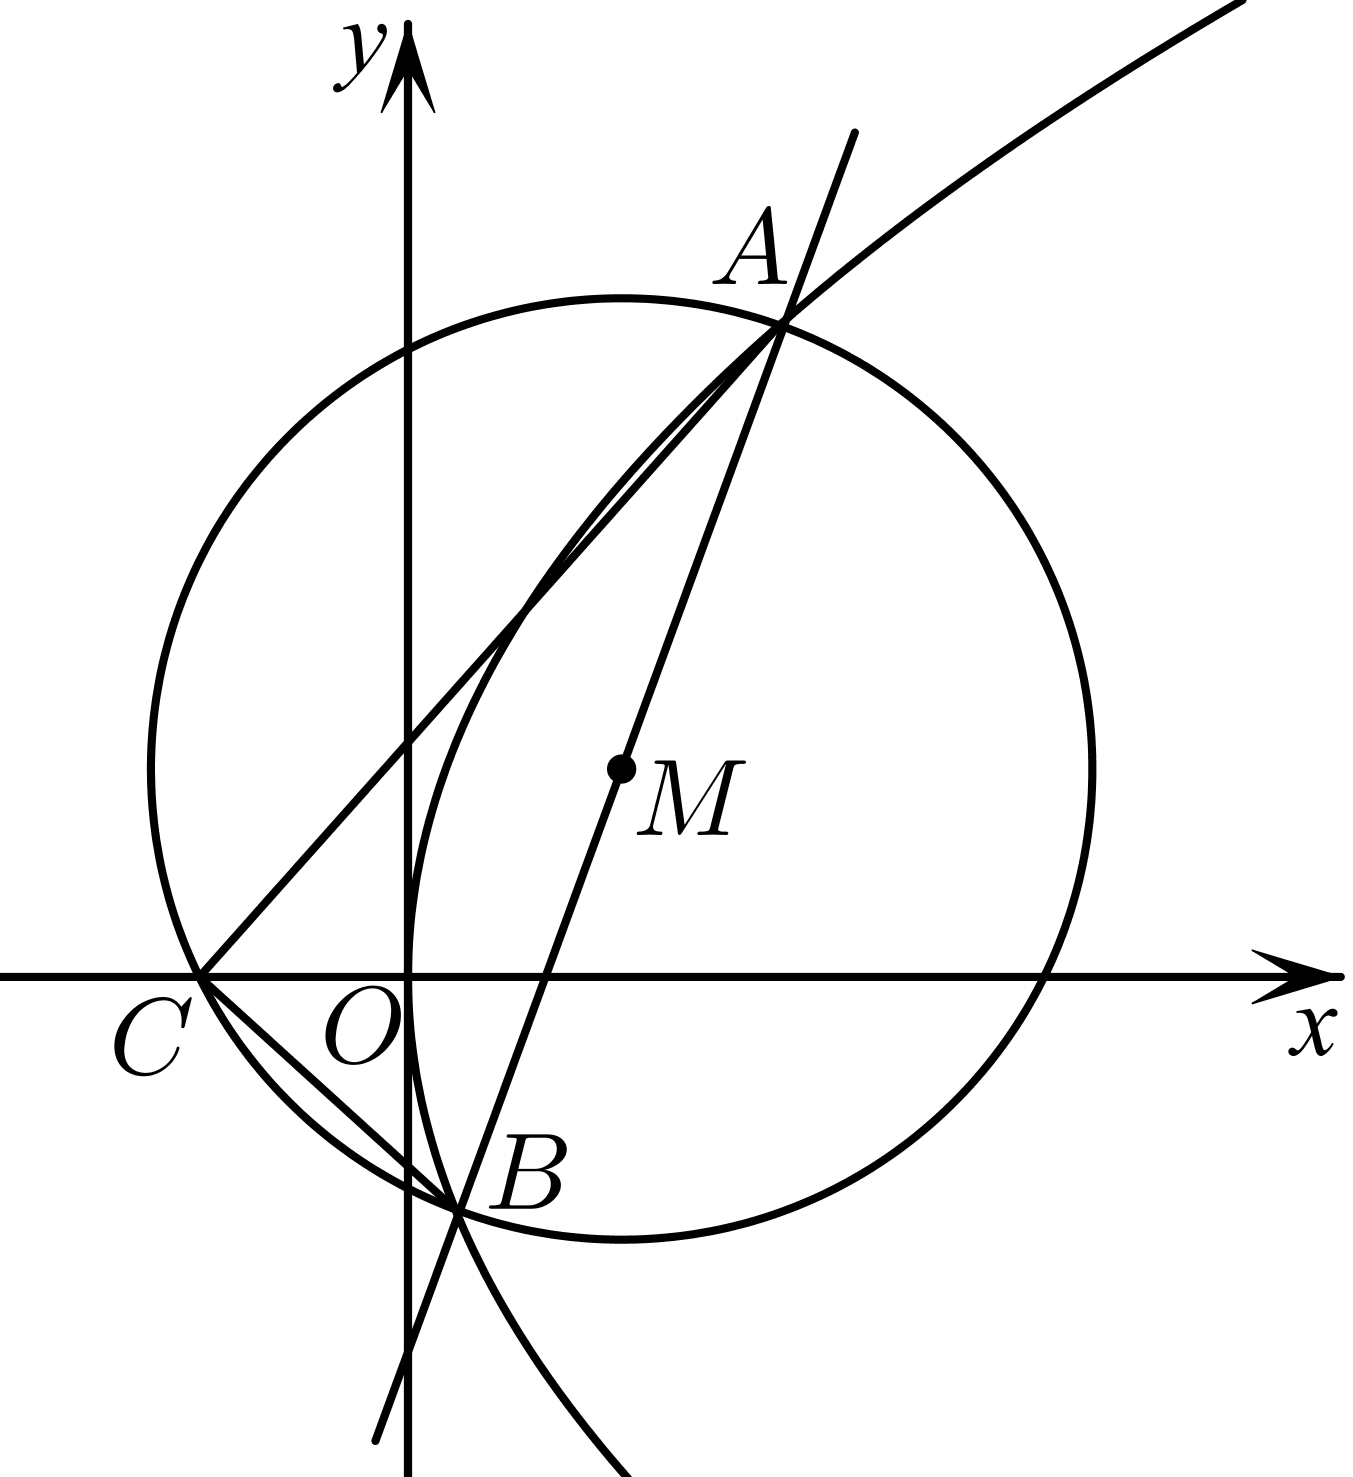
\includegraphics[width=38mm]{figs/18-12.png}}
\xiexwei{14mm}

{\ansblockgrayfalse
\begin{ansblock}[2章-练-课时18-12]
% ans:2章-练-课时18-12
\ansitem{13}{(1) y²=8x；(2) 存在，t=±√2/2}
\ansnote{详解}{(1) 设 \(y^{2}=ax\)，准线 \(x=-a/4=-2\)，得 \(a=8\)，故抛物线 \(y^{2}=8x\)．\par\noindent (2) 联立 \(x=ty+1\)：\(y^{2}-8ty-8=0\)，得 \(y_1+y_2=8t\)、\(y_1y_2=-8\)；\(x_1+x_2=t(y_1+y_2)+2=8t^{2}+2\)、\(x_1x_2=t^{2}y_1y_2+t(y_1+y_2)+1=1\)．设 \(C(x_0,0)\)（\(x_0<0\)）．\(C\) 在以 \(AB\) 为直径的圆上，故 \(\angle ACB=90^{\circ}\)，即 \(CA\cdot CB=0\)：\((x_1-x_0)(x_2-x_0)+y_1y_2=0\)，得 \(x_0^{2}-(8t^{2}+2)x_0+(x_1x_2+y_1y_2)=0\)，即 \(x_0^{2}-(8t^{2}+2)x_0-7=0\)（记为①）．内心在 \(x\) 轴上等价于 \(x\) 轴平分 \(\angle ACB\)，即 \(k_{CA}+k_{CB}=0\)：\(y_1(x_2-x_0)+y_2(x_1-x_0)=0\)，得 \(2ty_1y_2+(y_1+y_2)(1-x_0)=0\)，即 \(-16t+8t(1-x_0)=0\)，故 \(8t(-1-x_0)=0\)．\(t=0\) 时直线 \(x=1\) 垂直于 \(x\) 轴，与题设矛盾，舍；故 \(x_0=-1<0\)，代入①：\(1+(8t^{2}+2)-7=0\)，故 \(t^{2}=1/2\)，\(t=\pm\sqrt{2}/2\)．}
\end{ansblock}}

\tjdnr{三}{对称、多选与拼接综合}{例\textbf{14}}{难(知识点一)}{已知椭圆\(C\)：\(x^{2}/a^{2}+y^{2}/b^{2}=1\)（\(a>b>0\)）过点\((1,\sqrt{2}/2)\)，且焦距为2．}

\bindp (1) 求椭圆\(C\)的标准方程；

\bindp (2) 设过点\(P(-2,0)\)的直线\(l\)与椭圆\(C\)交于不同的两点\(A\)、\(B\)，点\(G(0,-1/2)\)，如果\(|GA|=|GB|\)，求直线\(l\)的方程．
\xiexwei{18mm}

{\ansblockgrayfalse
\begin{ansblock}[2章-练-课时18-13]
% ans:2章-练-课时18-13
\ansitem{14}{(1) x²/2+y²=1；(2) y=(2−√2)/2·(x+2) 或 y=0}
\ansnote{详解}{(1) 焦距为2，故 \(c=1\)、\(a^{2}=b^{2}+1\)；点 \((1,\sqrt{2}/2)\) 代入：\(1/a^{2}+(1/2)/b^{2}=1\)．令 \(u=b^{2}\)：\(1/(u+1)+1/(2u)=1\)，即 \(2u+(u+1)=2u(u+1)\)，整理得 \(2u^{2}-u-1=0\)，解得 \(u=1\)，故 \(a^{2}=2\)、\(b^{2}=1\)，椭圆 \(C\)：\(x^{2}/2+y^{2}=1\)．\par\noindent (2) 先取 \(y=0\)：\(A\)、\(B\) 为 \((\pm\sqrt{2},0)\)，\(G\) 在 \(y\) 轴上，\(|GA|=|GB|\) 成立，是一解．\(k\neq 0\) 时设 \(l\)：\(y=k(x+2)\)，联立 \(x^{2}+2y^{2}=2\)：\((1+2k^{2})x^{2}+8k^{2}x+8k^{2}-2=0\)，弦中点 \(M\)：\(x_M=-4k^{2}/(1+2k^{2})\)、\(y_M=k(x_M+2)=2k/(1+2k^{2})\)．\(|GA|=|GB|\) 等价于 \(GM\perp l\)，即 \(x_M+k(y_M+1/2)=0\)，两边乘 \(2(1+2k^{2})\)：\(-8k^{2}+4k^{2}+k(1+2k^{2})=0\)，即 \(k(2k^{2}-4k+1)=0\)（\(k\neq 0\)），故 \(k=(2\pm\sqrt{2})/2\)．两交点条件：\(\Delta=8-16k^{2}>0\)，即 \(k^{2}<1/2\)；\(k=(2+\sqrt{2})/2\) 时 \(k^{2}=(3+2\sqrt{2})/2>1/2\)，舍；\(k=(2-\sqrt{2})/2\) 时 \(k^{2}=(3-2\sqrt{2})/2<1/2\)，符合．故 \(l\)：\(y=(2-\sqrt{2})/2\cdot(x+2)\) 或 \(y=0\)．}
\end{ansblock}}

\liB{变式\textbf{15}}{中档(知识点一)}{}{如图，曲线\(C\)由上半椭圆\(C_1\)：\(y^{2}/a^{2}+x^{2}/b^{2}=1\)（\(a>b>0\)，\(y\geqslant 0\)）和部分抛物线\(C_2\)：\(y=-x^{2}+1\)（\(y\leqslant 0\)）连接而成，\(C_1\)与\(C_2\)的公共点为\(A\)、\(B\)，其中\(C_1\)的离心率为\(\sqrt{3}/2\)．}
\ansfig{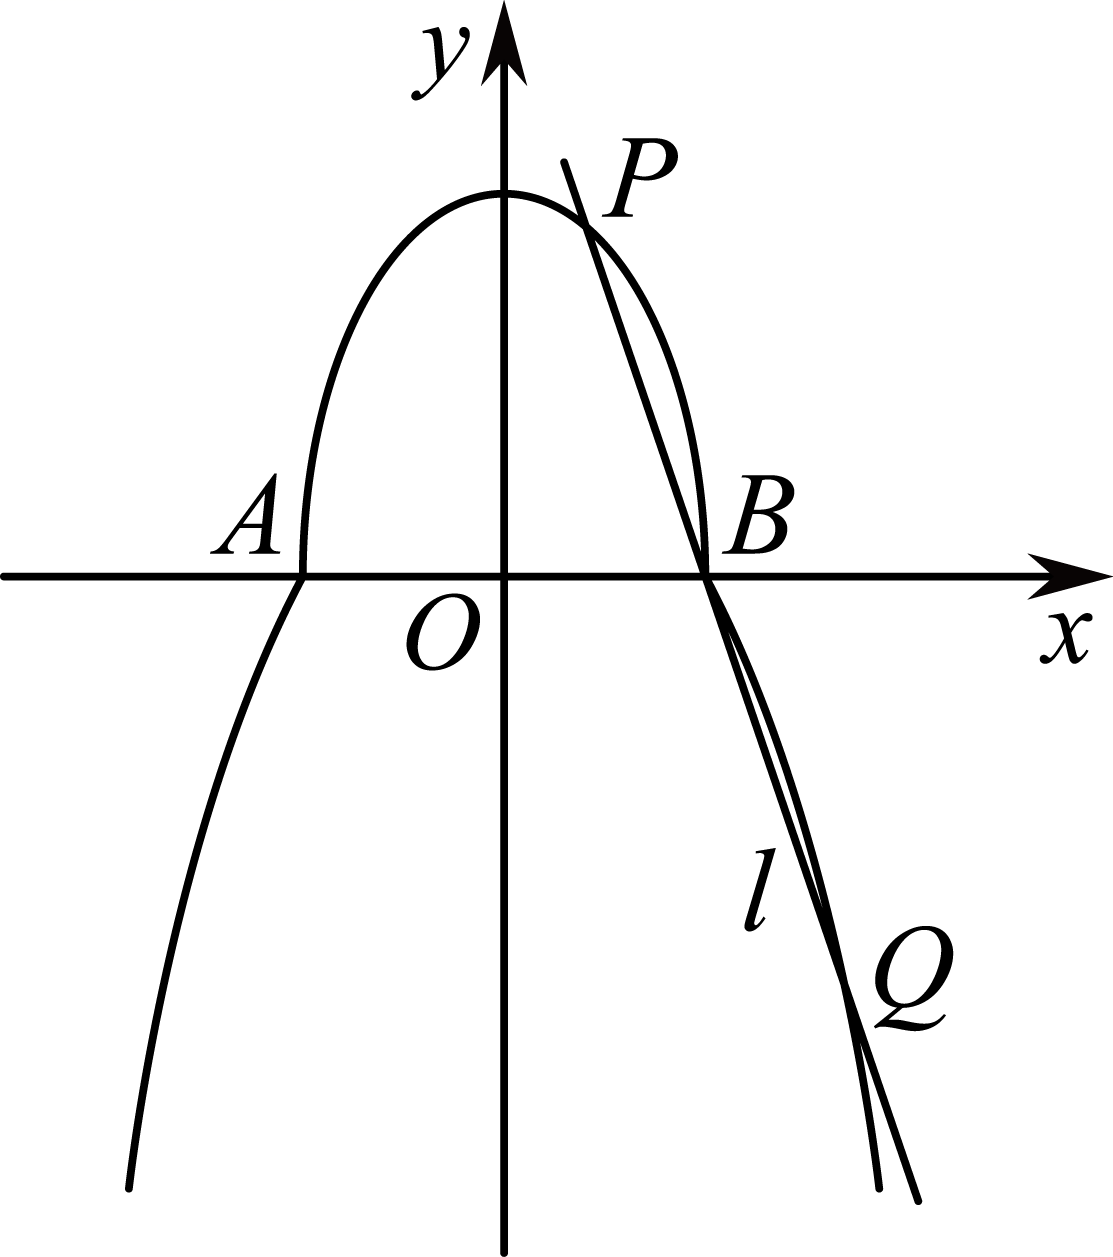
\includegraphics[width=38mm]{figs/18-14.png}}

\bindp (1) 求\(a\)、\(b\)的值；

\bindp (2) 过点\(B\)的直线\(l\)与\(C_1\)、\(C_2\)分别交于点\(P\)、\(Q\)（均异于点\(A\)、\(B\)），是否存在直线\(l\)，使得以\(PQ\)为直径的圆恰好过点\(A\)？若存在，求出直线\(l\)的方程；若不存在，请说明理由．
\xiexwei{18mm}

{\ansblockgrayfalse
\begin{ansblock}[2章-练-课时18-14]
% ans:2章-练-课时18-14
\ansitem{15}{(1) a=2、b=1；(2) 存在，8x+3y−8=0}
\ansnote{详解}{(1) \(C_2\) 与 \(x\) 轴交于 \((\pm 1,0)\)，即 \(A(-1,0)\)、\(B(1,0)\)，且 \(x^{2}/b^{2}=1\) 在 \(y=0\) 处成立，故 \(b=1\)．\(e=c/a=\sqrt{3}/2\)，故 \(c^{2}=3a^{2}/4\)；\(a^{2}-c^{2}=b^{2}=1\)，得 \(a^{2}/4=1\)，故 \(a=2\)．\par\noindent (2) \(C_1\)：\(y^{2}/4+x^{2}=1\)（\(y\geqslant 0\)）．设 \(l\)：\(y=k(x-1)\)（\(k\neq 0\)；\(k=0\) 时 \(l\) 与 \(x\) 轴重合，不合）．交 \(C_1\)：\((k^{2}+4)x^{2}-2k^{2}x+k^{2}-4=0\)，一根 \(x=1\)（点 \(B\)），故 \(x_P=(k^{2}-4)/(k^{2}+4)\)、\(y_P=k(x_P-1)=-8k/(k^{2}+4)\)．交 \(C_2\)：\(k(x-1)=-(x-1)(x+1)\)，故 \((x-1)(k+x+1)=0\)，\(x_Q=-k-1\)（\(x_Q\neq 1\)，故 \(k\neq -2\)）、\(y_Q=k(x_Q-1)=-k^{2}-2k\)．\par\noindent \(\overrightarrow{AP}=(2k^{2}/(k^{2}+4),-8k/(k^{2}+4))=(2k/(k^{2}+4))\cdot(k,-4)\)；\(\overrightarrow{AQ}=(-k,-k^{2}-2k)=-k(1,k+2)\)．以 \(PQ\) 为直径的圆过 \(A\) 等价于 \(AP\perp AQ\)，即 \(\overrightarrow{AP}\cdot\overrightarrow{AQ}=0\)：\((2k/(k^{2}+4))\cdot(-k)\cdot[k-4(k+2)]=0\)，\(k\neq 0\)，故 \(3k+8=0\)，\(k=-8/3\)．回验落位：\(y_P=48/25>0\)（\(P\) 在上半椭圆）、\(y_Q=-16/9\leqslant 0\)（\(Q\) 在下半抛物线），符合．故存在 \(l\)：\(y=-(8/3)(x-1)\)，即 \(8x+3y-8=0\)．}
\end{ansblock}}

\tjdnr{三}{对称、多选与拼接综合}{例\textbf{16}}{难(知识点二)}{设\(A\)、\(B\)为双曲线\(C\)：\(x^{2}/a^{2}-y^{2}/b^{2}=1\)（\(a>0\)，\(b>0\)）的左、右顶点，直线\(l\)过右焦点\(F\)且与双曲线\(C\)的右支交于\(M\)、\(N\)两点，当直线\(l\)垂直于\(x\)轴时，\(\triangle AMN\)为等腰直角三角形．}

\bindp (1) 求双曲线\(C\)的离心率；

\bindp (2) 已知\(|AB|=4\)，若直线\(AM\)、\(AN\)分别交直线\(x=a/2\)于\(P\)、\(Q\)两点，当直线\(l\)的倾斜角变化时，以\(PQ\)为直径的圆是否过定点，若过定点求出定点的坐标；若不过定点，请说明理由．
\xiexwei{18mm}

{\ansblockgrayfalse
\begin{ansblock}[2章-练-课时18-16]
% ans:2章-练-课时18-16
\ansitem{16}{(1) e=2；(2) 恒过定点 (4,0) 与 (−2,0)（两点同时在圆上）}
\ansnote{详解}{(1) \(l\perp x\) 轴时 \(M\)、\(N\) 的坐标为 \((c,\pm b^{2}/a)\)；\(A\) 在 \(x\) 轴上，\(|AM|=|AN|\) 自动成立，故直角顶点只能是 \(A\)（若直角在 \(M\)，\(MA\) 需水平，即 \(y_M=0\)，不可能），故 \(\angle MAN=90^{\circ}\)，\(k_{AM}=\pm 1\)，即 \(b^{2}/a=a+c\)，故 \(c^{2}-a^{2}=a^{2}+ac\)，即 \(e^{2}-e-2=0\)，得 \(e=2\)（负根舍）．\par\noindent (2) \(2a=4\)，故 \(a=2\)、\(c=2a=4\)、\(b^{2}=12\)，\(C\)：\(x^{2}/4-y^{2}/12=1\)，\(A(-2,0)\)，\(x=a/2=1\)．设 \(l\)：\(x=ty+4\)（\(t\) 为实数，\(t=0\) 即 \(l\perp x\) 轴亦含；\(|t|<1/\sqrt{3}\) 时与右支交两点）．代入得 \((3t^{2}-1)y^{2}+24ty+36=0\)，故 \(y_1y_2=36/(3t^{2}-1)\)、\(y_1+y_2=-24t/(3t^{2}-1)\)、\(x_1+x_2=t(y_1+y_2)+8=-8/(3t^{2}-1)\)、\(x_1x_2=t^{2}y_1y_2+4t(y_1+y_2)+16=(-12t^{2}-16)/(3t^{2}-1)\)．\par\noindent 直线 \(AM\) 过 \(A(-2,0)\)、\(M(x_1,y_1)\)，在 \(x=1\) 处 \(y=3y_1/(x_1+2)\)，故 \(P(1,p)\)、\(Q(1,q)\)，其中 \(p=3y_1/(x_1+2)\)、\(q=3y_2/(x_2+2)\)．而 \((x_1+2)(x_2+2)=x_1x_2+2(x_1+x_2)+4=(-12t^{2}-16-16+12t^{2}-4)/(3t^{2}-1)=-36/(3t^{2}-1)\)，故 \(pq=9y_1y_2/[(x_1+2)(x_2+2)]=9\cdot[36/(3t^{2}-1)]\cdot[(3t^{2}-1)/(-36)]=-9\)，与 \(t\) 无关．\par\noindent 以 \(PQ\) 为直径的圆：\((x-1)^{2}+(y-p)(y-q)=0\)，即 \((x-1)^{2}+y^{2}-(p+q)y+pq=0\)．令 \(y=0\)：\((x-1)^{2}=-pq=9\)，得 \(x=4\) 或 \(x=-2\)，即对每一条满足题设的 \(l\)，\((4,0)\) 与 \((-2,0)\) 同时在该圆上．特例回验：\(t=0\) 时 \(M\)、\(N\) 为 \((4,\pm 6)\)，\(P(1,3)\)、\(Q(1,-3)\)，圆 \((x-1)^{2}+y^{2}=9\)，两点均在圆上；\(3t^{2}-1=0\) 时 \(l\) 平行于渐近线仅一交点，不在题设内．}
\end{ansblock}}

\xiaojie{①识别：以内切圆圆心位置、中垂线等距（对称）条件反求参数或直线、过定点割线的多选判定、半椭圆＋抛物线拼接、等腰直角定位离心率后再问圆过定点等综合形态，判归本题型．}
\bindp {\kaishu ②操作：对称条件译成“角平分＝斜率和为零”或“等距＝垂直平分”；多选逐项独立验真伪，反例与特值优先；拼接曲线逐段求交并核验落位（各段定义域内）；高难小题先把特殊位置（通径、垂直）的信息转成 \(a,b,c\) 等式．}
\bindp {\kaishu ③收束：对称与存在性求出参数后回验两交点不同且落位正确；拼接问题回验交点分段归属；定点问题区分“或”与“且”，说明定点对全部允许参数成立．}

% ============================================================
% 课堂评价 G5（恒5＝3单选+2填空＝导槽 G1~G5；ketang 新制顺排可跨栏，禁 \vbox 装栏）
% 印面号 17—21；多选门：本片课堂评价无多选，全片 1（印12）≤4 合规
% ============================================================
\begin{ketang}{本组共5题（第17—21题），17—19为单选，20—21为填空．}

\jiancestem{{\fontsize{11.4pt}{14pt}\selectfont\heihao {\numboldjian 17}．}\hspace{4.1mm}\tieside{简单(知识点一)}\hspace{2.2mm}已知抛物线\(C\)：\(y^{2}=2px\)（\(p>0\)）的焦点为\(F\)，过\(F\)作直线\(l\)交抛物线\(C\)于\(M\)、\(N\)两点，与抛物线的准线交于点\(P\)，若\(|PM|=2|PF|\)，则直线\(l\)的倾斜角为\nobreak(\kongwei)}

\bindopt {\fontsize{10.5pt}{\qpTJgLeadPingjia}\selectfont \makebox[\dimexpr0.5\linewidth-1em\relax][l]{A．\(\pi/6\)或\(5\pi/6\)}\makebox[\dimexpr0.5\linewidth-1em\relax][l]{B．\(\pi/4\)或\(3\pi/4\)}\par}

\bindopt {\fontsize{10.5pt}{\qpTJgLeadPingjia}\selectfont \makebox[\dimexpr0.5\linewidth-1em\relax][l]{C．\(\pi/3\)或\(2\pi/3\)}\makebox[\dimexpr0.5\linewidth-1em\relax][l]{D．\(\pi/2\)}\par}

{\ansblockgrayfalse
\begin{ansblock}[2章-导-课时18-G1]
% ans:2章-导-课时18-G1
\ansitem{17}{C}
\ansnote{详解}{\(F(p/2,0)\)，准线 \(x=-p/2\)，记准线与 \(x\) 轴交点 \(A(-p/2,0)\)，\(|AF|=p\)．\(l\) 过 \(F\) 与准线交于 \(P\)，弦 \(MN\) 过 \(F\)，沿直线点序为 \(P\)、\(N\)、\(F\)、\(M\)（\(N\) 近 \(F\)、\(M\) 远 \(F\)，\(|PN|<|PF|<|PM|\)）．由 \(|PM|=2|PF|\) 及 \(|PM|=|PF|+|FM|\) 得 \(|FM|=|PF|\)，即 \(F\) 为 \(PM\) 中点．过 \(M\) 作 \(MB\perp\) 准线于 \(B\)，由定义 \(|FM|=|BM|\)；\(A\) 为 \(PB\) 中点（\(P\)、\(B\) 同在准线上，纵坐标和为0）、\(F\) 为 \(PM\) 中点，故 \(AF\) 为 \(\triangle PMB\) 中位线，\(|BM|=2|AF|=2p\)，故 \(|FM|=|PF|=2p\)．\(P\) 与 \(F\) 的水平距离为 \(p\)，设倾斜角 \(\theta\)，则 \(|PF|\cdot|\cos\theta|=p\)，故 \(2p|\cos\theta|=p\)，\(|\cos\theta|=1/2\)，\(\theta\in(0,\pi)\)，得 \(\theta=\pi/3\) 或 \(\theta=2\pi/3\)．故选：C．\par\noindent 特例回验：取 \(p=2\)（\(y^{2}=4x\)）、\(\theta=\pi/3\)，\(l\)：\(y=\sqrt{3}(x-1)\)，联立得 \(3x^{2}-10x+3=0\)，\(M(3,2\sqrt{3})\)、\(N(1/3,-2\sqrt{3}/3)\)、\(P(-1,-2\sqrt{3})\)；\(|PF|=\sqrt{4+12}=4\)、\(|PM|=\sqrt{16+48}=8\)，\(|PM|=2|PF|\) 且 \(|FM|=x_M+1=4=|PF|\)，符合；\(\theta=2\pi/3\) 与 \(\pi/3\) 关于 \(x\) 轴对称，同成立．}
\end{ansblock}}

\jiancestem{{\fontsize{11.4pt}{14pt}\selectfont\heihao {\numboldjian 18}．}\hspace{4.1mm}\tieside{简单(知识点一)}\hspace{2.2mm}已知椭圆\(x^{2}/4+y^{2}/3=1\)的左、右焦点分别为\(F_1\)、\(F_2\)，过\(F_2\)且垂直于长轴的直线交椭圆于\(A\)、\(B\)两点，则\(\triangle ABF_1\)内切圆的半径为\nobreak(\kongwei)}

\bindopt {\fontsize{10.5pt}{\qpTJgLeadPingjia}\selectfont \makebox[\dimexpr0.25\linewidth-0.5em\relax][l]{A．\(4/3\)}\makebox[\dimexpr0.25\linewidth-0.5em\relax][l]{B．\(1\)}\makebox[\dimexpr0.25\linewidth-0.5em\relax][l]{C．\(4/5\)}\makebox[\dimexpr0.25\linewidth-0.5em\relax][l]{D．\(3/4\)}\par}

\begin{ansblock}[2章-导-课时18-G2]
% ans:2章-导-课时18-G2
\ansitem{18}{D}
\ansnote{详解}{\(a=2\)、\(b=\sqrt{3}\)，故 \(c=\sqrt{4-3}=1\)，\(F_2(1,0)\)．通径：\(x=1\) 代入得 \(y^{2}=3(1-1/4)=9/4\)，\(|y|=3/2\)，故 \(|AB|=3\)（\(=2b^{2}/a=3\)，两法互证）．以 \(|F_1F_2|=2\) 为底：\(S_{\triangle ABF_1}=|AB|\cdot 2/2=3\)．周长：\(|AF_1|+|BF_1|=(2a-|AF_2|)+(2a-|BF_2|)=8-|AB|=5\)，故周长为 \(5+3=8\)．内切圆半径 \(r=2\times 3/8=3/4\)．故选：D．}
\end{ansblock}

\jiancestem{{\fontsize{11.4pt}{14pt}\selectfont\heihao {\numboldjian 19}．}\hspace{4.1mm}\tieside{简单(知识点一)}\hspace{2.2mm}过点\((0,-2)\)的直线与抛物线\(y^{2}=8x\)交于\(A\)、\(B\)两点，若线段\(AB\)中点的横坐标为2，则\(|AB|=\)\nobreak(\kongwei)}

\bindopt {\fontsize{10.5pt}{\qpTJgLeadPingjia}\selectfont \makebox[\dimexpr0.25\linewidth-0.5em\relax][l]{A．\(2\sqrt{17}\)}\makebox[\dimexpr0.25\linewidth-0.5em\relax][l]{B．\(\sqrt{17}\)}\makebox[\dimexpr0.25\linewidth-0.5em\relax][l]{C．\(2\sqrt{15}\)}\makebox[\dimexpr0.25\linewidth-0.5em\relax][l]{D．\(\sqrt{15}\)}\par}

{\ansblockgrayfalse
\begin{ansblock}[2章-导-课时18-G3]
% ans:2章-导-课时18-G3
\ansitem{19}{C}
\ansnote{详解}{设直线 \(y=kx-2\)（过 \((0,-2)\)），\(A(x_1,y_1)\)、\(B(x_2,y_2)\)．代入 \(y^{2}=8x\)：\(k^{2}x^{2}-4(k+2)x+4=0\)，\(\Delta=16(k+2)^{2}-16k^{2}=64(k+1)>0\)，故 \(k>-1\)．中点横坐标 \((x_1+x_2)/2=2(k+2)/k^{2}=2\)，故 \(k^{2}=k+2\)，即 \(k^{2}-k-2=0\)，得 \(k=2\) 或 \(k=-1\)；\(k=-1\) 时 \(\Delta=0\)（相切不成弦），舍，故 \(k=2\)．此时 \(x^{2}-4x+1=0\)，\(x_1+x_2=4\)、\(x_1x_2=1\)，弦长 \(|AB|=\sqrt{1+k^{2}}\cdot\sqrt{(x_1+x_2)^{2}-4x_1x_2}=\sqrt{5}\cdot\sqrt{12}=2\sqrt{15}\)．故选：C．}
\end{ansblock}}

\jiancestem{{\fontsize{11.4pt}{14pt}\selectfont\heihao {\numboldjian 20}．}\hspace{4.1mm}\tieside{简单(知识点一)}\hspace{2.2mm}过椭圆\(x^{2}/16+y^{2}/9=1\)的右焦点\(F\)作与\(x\)轴垂直的直线，与椭圆交于\(A\)、\(B\)两点，则以\(AB\)为直径的圆的面积是\kongbai{}．}
\xiexwei{7mm}

\begin{ansblock}[2章-导-课时18-G4]
% ans:2章-导-课时18-G4
\ansitem{20}{81π/16}
\ansnote{详解}{\(a=4\)、\(b=3\)，故 \(c=\sqrt{16-9}=\sqrt{7}\)，\(F(\sqrt{7},0)\)．\(x=\sqrt{7}\) 代入：\(y^{2}=9(1-7/16)=81/16\)，\(|y|=9/4\)，故 \(|AB|=9/2\)（与通径 \(2b^{2}/a=18/4=9/2\) 一致）．圆半径 \(r=|AB|/2=9/4\)，面积 \(S=\pi r^{2}=81\pi/16\)．}
\end{ansblock}

\jiancestem{{\fontsize{11.4pt}{14pt}\selectfont\heihao {\numboldjian 21}．}\hspace{4.1mm}\tieside{简单(知识点一)}\hspace{2.2mm}设\(F\)为抛物线\(C\)：\(y^{2}=3x\)的焦点，过\(F\)且倾斜角为\(30^{\circ}\)的直线交\(C\)于\(A\)、\(B\)两点，\(O\)为坐标原点，则\(\triangle ABO\)的面积为\kongbai{}．}
\xiexwei{7mm}

\begin{ansblock}[2章-导-课时18-G5]
% ans:2章-导-课时18-G5
\ansitem{21}{9/4}
\ansnote{详解}{\(2p=3\)，故 \(p=3/2\)，\(F(3/4,0)\)，\(k=\tan 30^{\circ}=\sqrt{3}/3\)，直线 \(y=(\sqrt{3}/3)(x-3/4)\)．代入 \(y^{2}=3x\)：\((x-3/4)^{2}=9x\)，即 \(x^{2}-(21/2)x+9/16=0\)（\(\Delta=441/4-9/4=108>0\)），\(x_1+x_2=21/2\)．由抛物线定义 \(|AB|=x_1+x_2+p=21/2+3/2=12\)．\(O\) 到直线 \(AB\)（即 \(\sqrt{3}x-3y-3\sqrt{3}/4=0\)）的距离 \(d=(3\sqrt{3}/4)/\sqrt{3+9}=3/8\)，故 \(S_{\triangle ABO}=|AB|\cdot d/2=12\times(3/8)/2=9/4\)．}
\end{ansblock}

\end{ketang}

% ---- 尾块（\tailfill 置 \end{multicols} 前；无参＝内容尾随框，件侧不擅自定高） ----
\tailfill

\end{multicols}
\end{document}
